\begin{activity} \label{A:1.7.2}
This activity builds on your work in Preview Activity~\ref{PA:1.7}, using the same function $f$ as given by the graph that is repeated in Figure~\ref{F:1.7.A2}
\begin{figure}[h]
\begin{center}
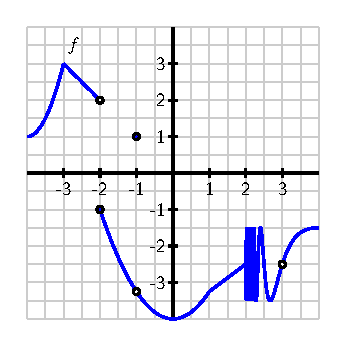
\includegraphics{figures/1_7_PA1.eps}
\caption{The graph of $y = f(x)$ for Activity~\ref{A:1.7.2}.} \label{F:1.7.A2}
\end{center}
\end{figure}
\ba
	\item At which values of $a$ does $\lim_{x \to a} f(x)$ not exist?
	\item At which values of $a$ is $f(a)$ not defined?
	\item At which values of $a$ does $f$ have a limit, but $\lim_{x \to a} f(x) \ne f(a)$?
	\item State all values of $a$ for which $f$ is not continuous at $x = a$.
	\item Which condition is stronger, and hence implies the other:   $f$  has a limit at $x = a$ or  $f$ is continuous at $x = a$?  Explain, and hence complete the following sentence:  ``If $f$ \underline{\hspace{1.5in}} at $x = a$, then $f$ \underline{\hspace{1.5in}} at $x = a$,'' where you complete the blanks with \emph{has a limit} and \emph{is continuous}, using each phrase once.
\ea
\end{activity}
\begin{smallhint}
\ba
	\item Consider the left- and right-hand limits at each value.
	\item Carefully examine places on the graph where there's an open circle.
	\item Are there locations on the graph where the function has a limit but there's a hole in the graph?
	\item Remember that at least one of three conditions must fail: if the function lacks a limit, if the function is undefined, or if the limit exists but does not equal the function value, then $f$ is not continuous at the point.
	\item Note that the definition of being continuous requires the limit to exist.
\ea
\end{smallhint}
\begin{bighint}
\ba
	\item Consider the left- and right-hand limits at each value, and recall that they must both exist and be equal in order for the overall limit to exist.
	\item Carefully examine places on the graph where there's an open circle; at such locations, look vertically to see if the function has an assigned value at that point.
	\item Are there locations on the graph where the function has a limit but there's a hole in the graph?
	\item Remember that at least one of three conditions must fail: if the function lacks a limit, if the function is undefined, or if the limit exists but does not equal the function value, then $f$ is not continuous at the point.
	\item Note that the definition of being continuous requires the limit to exist.
\ea
\end{bighint}
\begin{activitySolution}
\ba
	\item $\lim_{x \to a} f(x)$ does not exist at $a = -2$ since $\lim_{x \to -2^-} f(x) = 2 \ne -1 = \lim_{x \to -2^+}$ and $\lim_{x \to a} f(x)$ does not exist at $a = +2$ since $\lim_{x \to 2^+} f(x)$ does not exist due to the infinitely oscillatory behavior of $f$.
	\item The only point at which $f$ is not defined is at $a = 3$.
	\item At $x = -1$, note that $\lim_{x \to -1} f(x)$ exists (and appears to have value approximately $-3.25$), but $f(-1) = 1$, and thus $\lim_{x \to -1} f(x) \ne f(-1)$.  At $x = 3$, $\lim_{x \to 3} f(x) = -2.5$, but $f(3)$ is not defined, so the limit exists but does not equal the function value.
	\item Based on our work in (a), (b), and (c), $f$ is not continuous at $a=-2$ and $a = 2$ because $f$ does not have a limit at those points; $f$ is not continuous at $a = 3$ since $f$ is not defined there; and $f$ is not continuous at $a = -1$ because at that point its limit does not equal its function value.
	\item ``If $f$ \underline{is continuous} at $x = a$, then $f$ \underline{has a limit} at $x = a$,'' since one of the defining properties of ``being continuous'' at $x = a$ is that the function has a limit at that input value.  This shows that being continuous is a stronger condition than having a limit.
\ea
\end{activitySolution}
\aftera